\chapter{Testen}\label{ch:testen}

%% Machen Sie sich auf Basis Ihrer Überlegungen zur Qualitätssicherung Gedanken darüber,
%% wie Sie die Erfüllung der Anforderungen möglichst automatisiert im Rahmen von Teststufen
%% (Unit-Test, Komponententest, Integrationstest, Systemtest, Regressionstest und Abnahmetest)
%% überprüfen werden.


\section{Testplan}\label{sec:testplan}

%% Definieren Sie Zeitpunkte für die jeweiligen Teststufen in Ihrer Projektplanung.
%% Dazu können Sie die Meilensteine zu Hilfe nehmen.
%% Überlegen Sie, wie die Test-Architektur der jeweiligen Teststufen aussehen.
%% Verwenden Sie Testmethoden wie z.B.

%% Grenzwertanalyse
%% 100% Zustandsabdeckung
%% 100% Transitionsüberdeckung
%% Pfadüberdeckung
%% Tiefensuche
%% Breitensuche

%% Versuchen Sie, so gut wie möglich, Ihre Tests zu automatisieren.

\subsection{Unit-Test}\label{subsec:unit-tests}
Für jede neu implementierte Klasse wurden direkt während der Implementation Unit-Tests realisiert.
Automatisiert wurden die Tests mit dem GTest-Framework.
Bei den Tests wird jede Funktionalität der öffentlichen Schnittstelle einer getesteten Einheit überprüft.
Automatisiert getestet wurden alle State-Machines \ref{subsec:stm-tests}, das Datenmodell, der EmbeddedRecorder, das parsen von Startargumenten
das Eventsystem mitsamt des Dispatchers, sowie der für die interne Funktionalität der State-Machines benötigte Timer.
Besonderes umfassend wurde neben sicherheitskritischer Funktionalität, auch die Verwaltung der \glspl{workpiece} im Datenmodell getestet,
da Fehler an diese Stelle kritisch für den korrekten Sortierprozess sind.
Hierfür wurden konkrete abläufe mit unterschiedlichen \glspl{workpiece} simuliert
und das Datenmodell auf korrektes Verhalten kontrolliert.
Das Testen der HAL wird in \ref{subsec:hal-tests} erläutert.
Eine Ausgabe der Ausführung der Unit-Tests ist in \ref{fig:unit-test-execution} zu finden.
Aus Gründen der Übersichtlichkeit sind die Tests der State-Machines, die durch die Abdeckungbäume in \ref{sec:abdeckungsbaueme} beschrieben werden, in diesem Protokoll eingeklappt.


\subsection{STM-Tests}\label{subsec:stm-tests}

\subsubsection{Implementation}
Im \textit{StmTestClient} werden die von der STM über das Interface \textit{IEventSender}
verschickten Events zwischengespeichert, sodass im Test
sichergestellt werden kann, dass an einer Transition genau die erwarteten Events (und keine weiteren)
verschickt werden.
Die Klasse ist in Abbildung~\ref{fig:cd_basis_stm_test} dargestellt.
Die Klasse \textit{StmTestBase} ist eine Basis-Klasse für \textit{gtest} Test-Fixtures,
und stellt die STMs inkl.\ Datenmodel und entsprechende Testmethoden zur Verfügung.
Der Parameter \textit{trigger} ist bei den Methoden das Event, welches eine Transition auslöst.
Die Liste an Events sind jene, die durch das Ausführen der Transition erzeugt werden sollen.

\begin{figure}[h]
    \centering
    \includegraphics[scale=0.5]{../out/diagrams/stage3/cd_stm_test}
    \caption{Basisklasse für Unit tests der STMs}
    \label{fig:cd_basis_stm_test}
\end{figure}


\section{Abdeckungsbäume}\label{sec:abdeckungsbaueme}

%% <konkrete Beschreibungen der Test Szenarien. Bei Bedarf die Tabelle vervielfältigen>
Für jede implementierte State-Machine wurden Unit-Tests geschrieben.
Diese Tests basieren auf den Abdeckungsbaum der jeweiligen State-Machine.
Mithilfe der Abdeckungsbäume wird sichergestellt, dass jeder Zustand getestet wird.
Dementsprechend wird auch ein möglichst großer Abdeckungsgrad sichergestellt.

\begin{figure}
    \makebox[\textwidth][c]{\includegraphics[width=1.25\textwidth]{../out/diagrams/stage3/tt_operation_manager}}
    \caption{Abdeckungsbaum der STM operation\_manager
        (Abbildung~\ref{fig:stm_operation_manager})}
    \label{fig:tt_operation_manager}
\end{figure}

\begin{figure}
    \makebox[\textwidth][c]{\includegraphics[width=1.25\textwidth]{../out/diagrams/stage3/tt_recieve_workpiece}}
    \caption{Abdeckungsbaum der STM receive\_workpiece
        (Abbildung~\ref{fig:stm_recieve_workpiece})}
    \label{fig:tt_recieve_workpiece}
\end{figure}

\begin{figure}
    \makebox[\textwidth][c]{\includegraphics[scale=0.5]{../out/diagrams/stage3/tt_height_measurement}}
    \caption{Abdeckungsbaum der STM height\_measurement
        (Abbildung~\ref{fig:stm_hoehe_messen})}
    \label{fig:tt_height_measurement}
\end{figure}

\begin{figure}
    \makebox[\textwidth][c]{\includegraphics[scale=0.5]{../out/diagrams/stage3/tt_sort_workpiece}}
    \caption{Abdeckungsbaum der STM sort\_workpiece
        (Abbildung~\ref{fig:stm_sort_workpiece})}
    \label{fig:tt_sort_workpiece}
\end{figure}

\begin{figure}
    \makebox[\textwidth][c]{\includegraphics[scale=0.5]{../out/diagrams/stage3/tt_workpiece_transfer}}
    \caption{Abdeckungsbaum der STM workpiece\_transfer
        (Abbildung~\ref{fig:stm_workpiece_transfer})}
    \label{fig:tt_workpiece_transfer}
\end{figure}

\begin{figure}
    \makebox[\textwidth][c]{\includegraphics[scale=0.5]{../out/diagrams/stage3/tt_workpiece_transfer_request}}
    \caption{Abdeckungsbaum der STM workpiece\_transfer\_request
        (Abbildung~\ref{fig:stm_workpiece_transfer_request})}
    \label{fig:tt_workpiece_transfer_request}
\end{figure}

\begin{figure}
    \makebox[\textwidth][c]{\includegraphics[scale=0.5]{../out/diagrams/stage3/tt_error_listener}}
    \caption{Abdeckungsbaum der STM error\_listener
        (Abbildung~\ref{fig:stm_error_listener})}
    \label{fig:tt_error_listener}
\end{figure}


\FloatBarrier
\section{Abnahmetests und Integrationstests}\label{sec:abnahmetest}

%% 6.3	Abnahmetest
%% Leiten Sie die Abnahmebedingungen aus den Kunden-Anforderungen her.
%% Dokumentieren Sie hier, welche Schritte für die Abnahme erforderlich sind
%% und welches Ergebnis jeweils erwartet wird (Test Cases).
%\begin{abntest}{Sortierung, Kapazität}{
    \refreq{1},
    \refreq{2},
    \refreq{3},
    \refreq{5},
    \refreq{13}, %<- TODO auslagern
    \refreq{30},
    \refreq{38},
    \refreq{39}
}{
    \item Das System befindet sich im Betriebszustand
    \item Falls nicht anders spezifiziert soll sichergestellt werden, dass
    \begin{enumerate}
        \item die \glspl{rampe}kapazität während der Tests nicht ausgeschöpft wird
        \item sich die \glspl{workpiece} während der Tests nicht überschlagen
    \end{enumerate}
}
    \label{abntest-sortierung-kapazitaet}

    \begin{ablauf}{Korrekte Reihenfolge}
        \item \Glspl{workpiece} in korrekter Reihenfolge einlegen:
        \begin{enumerate}[noitemsep, nolistsep]
            \item \gls{workpiece_metall}
            \item \gls{workpiece_bohrung}
            \item \gls{workpiece_flach}
            \item \gls{workpiece_metall}
        \end{enumerate}
    \end{ablauf}

    \erwartung
    Am Ende von \gls{anlage} 2 kommen die \Glspl{workpiece} in
    unveränderter Reihenfolge an (\refreq{2})

    \begin{ablauf}{Falsche Reihenfolge}
        \item Eine \gls{anlage} mit \gls{weiche}, die andere mit \gls{ejector} ausstatten
        (\refreq{30}, \refreq{38}, \refreq{39})
        \item \Glspl{workpiece} in falscher Reihenfolge einlegen:\label{enm:reih1}
        \begin{enumerate}[noitemsep, nolistsep]
            \item \gls{workpiece_hoch} %x
            \item \gls{workpiece_metall}
            \item \gls{workpiece_metall} %x
            \item \gls{workpiece_bohrung}
            \item \gls{workpiece_hoch} %x
            \item \gls{workpiece_flach}
            \item \gls{workpiece_bohrung} %x
            \item \gls{workpiece_metall}
        \end{enumerate}
        \item \Glspl{rampe}kapazität von \gls{anlage} 1 manuell ausschöpfen\label{enm:rampe1-voll}
        \item \Glspl{workpiece} in gleicher Reihenfolge wie in
        Schritt~\ref{enm:reih1} einlegen\label{enm:reih2}
        \item \Glspl{rampe}kapazität von \gls{anlage} 2 manuell ausschöpfen\label{enm:rampe2-voll}
    \end{ablauf}

    \erwartung
    \begin{enumerate}
        \item Bei Schritt~\ref{enm:reih1} und~\ref{enm:reih2}: Am Ende von \gls{anlage} 2 kommen
        \Glspl{workpiece} in folgender Reihenfolge an,
        alle anderen wurden aussortiert (\refreq{3})
        \begin{enumerate}[noitemsep, nolistsep]
            \item \gls{workpiece_metall}
            \item \gls{workpiece_bohrung}
            \item \gls{workpiece_flach}
            \item \gls{workpiece_metall}
        \end{enumerate}
        \item Nach Schritt~\ref{enm:rampe1-voll}  blinkt die gelbe \gls{ampelled}
        von \gls{anlage} 1 (\refreq{5}, \refreq{13})
        \item Nach Schritt~\ref{enm:rampe2-voll}  blinkt die gelbe \gls{ampelled}
        von \gls{anlage} 2 (\refreq{5}, \refreq{13})
    \end{enumerate}
    %todo: req 47 , 6
\end{abntest}

\abntest{Zustandsanzeigen}{
    \refreq{10},
    \refreq{11},
    \refreq{19},
    \refreq{45}
}{
    \item Das System befindet sich im Idle
}
\label{abntest-zustandsanzeigen}
\begin{anmerkungen}
    \item Die Anzeige von Fehlerzuständen wird in Abschnitt~\ref{abntest-fehlerumgang} getestet.
\end{anmerkungen}

\begin{ablauf}{Betriebszustände}
    \item \label{itm:to-service} Den Servicemodus betreten
    \item \label{itm:to-idle} Auf Rückkehr in den Idle warten
    \item \label{itm:to-betriebsz} Den Betriebszustand betreten
    \item \label{itm:to-idle2} Den Betriebszustand verlassen
\end{ablauf}
\begin{erwartung}
    \item Vor Schritt~\ref{itm:to-service} leuchten
    beide gelben \glspl{ampelled} dauerhaft, alle anderen sind aus (\refreq{45})
    \item Nach Schritt~\ref{itm:to-service} blinken
    beide grünen \glspl{ampelled}, alle anderen sind aus (\refreq{11})
    \item Nach Schritt~\ref{itm:to-idle} leuchten
    beide gelben \glspl{ampelled} dauerhaft, alle anderen sind aus (\refreq{45})
    \item Nach Schritt~\ref{itm:to-betriebsz} leuchten
    beide grünen \glspl{ampelled} dauerhaft, alle anderen sind aus (\refreq{10}, \refreq{19})
    \item Nach Schritt~\ref{itm:to-idle2} leuchten
    beide gelben \glspl{ampelled} dauerhaft, alle anderen sind aus (\refreq{45})
\end{erwartung}

\abntest{Fehlerumgang und Zustandsanzeigen}{
    \refreq{37},
    \refreq{43},
    \refreq{46} (indirekt durch \refreq{37}),
    \refreq{48}
}{
    \item Das System befindet sich im Idle
}
\label{abntest-fehlerumgang}

\begin{anmerkungen}
    \item Fehler erzeugen ist in diesem Abnahmetest wie folgt definiert:
    \begin{enumerate}
        \item In den Betriebszustand wechseln
        \item Kapazität beider \glspl{rampe} ausschöpfen
        \item Ein \gls{workpiece_hoch} einlegen
        \item Warten bis das \gls{workpiece_hoch} die \gls{lb_sw} erreicht
    \end{enumerate}
\end{anmerkungen}

\begin{ablauf}{Anstehened quittiert}
    \item \label{itm:1err} Fehler erzeugen
    \item\label{itm:1quitt} \gls{t_reset} drücken
    \item\label{itm:1ok} Die \gls{rampe} von \gls{anlage} 2 leeren
\end{ablauf}
\begin{erwartung}
    \item Nach Schritt~\ref{itm:1err}
    \begin{enumerate}
        \item bleiben die \glspl{belt} beider \glspl{anlage} stehen (\refreq{43})
        \item stehen beide \glspl{weiche} auf \gls{discard} (\refreq{48})
        \item blinkt die rote \gls{ampelled} schnell (\refreq{37}-\ref{req-37-unq})
    \end{enumerate}
    \item Nach Schritt~\ref{itm:1quitt} leuchtet die rote \gls{ampelled} dauerhaft (\refreq{37}-\ref{req-37-quit})
    \item Nach Schritt~\ref{itm:1ok} ist die rote \gls{ampelled} ausgeschaltet (\refreq{37}-\ref{req-37-ok})
\end{erwartung}

\begin{ablauf}{Gegangen unquittiert}
    \item \label{itm:2err} Fehler erzeugen
    \item\label{itm:2gegang} Die \gls{rampe} von \gls{anlage} 2 leeren
    \item\label{itm:2ok} \gls{t_reset} drücken
\end{ablauf}
\begin{erwartung}
    \item Nach Schritt~\ref{itm:2err}
    \begin{enumerate}
        \item bleiben die \glspl{belt} beider \glspl{anlage} stehen (\refreq{43})
        \item stehen beide \glspl{weiche} auf \gls{discard} (\refreq{48})
        \item blinkt die rote \gls{ampelled} schnell (\refreq{37}-\ref{req-37-unq})
    \end{enumerate}
    \item Nach Schritt~\ref{itm:2gegang} blinkt die rote \gls{ampelled} langsam (\refreq{37}-\ref{req-37-geg})
    \item Nach Schritt~\ref{itm:2ok} ist die rote \gls{ampelled} ausgeschaltet (\refreq{37}-\ref{req-37-ok})
\end{erwartung}

% TODO Fehler während quittiert oder unquittiert vorkommen lassen.

Die Abnahmetests wurden so detalliert gestaltet, dass sie sämtliche Funktionalität
des Softwaresystems abdecken und somit auch die Integrationstests darstellen.
Eine genaue Beschreibung des Ablaufes der einzelnen Abnahmetests findet sich in


\section{Testprotokolle und Auswertungen}\label{sec:testprotokolle-und-auswertungen}

%% Hier fügen Sie die Test Protokolle bei, auch wenn Fehler bereits beseitigt worden sind,
%% ist es schön zu wissen, welche Fehler einst aufgetaucht sind.
%% Eventuelle Anmerkung zur Fehlerbehandlung kann für weitere Entwicklungen hilfreich sein.
%% Das letzte Testprotokoll ist das Abnahmeprotokoll, das bei der abschließenden Vorführung erstellt wird.
%% Es enthält eine Auflistung der erfolgreich vorgeführten Funktionen des Systems
%% sowie eine Mängelliste mit Erklärungen der Ursachen der Fehlfunktionen und  Vorschlägen zur Abhilfe
In diesem Kapitel sind die Abnahmetests, Unit-Test Ergebnisse und die Tests für die Hal zu finden.

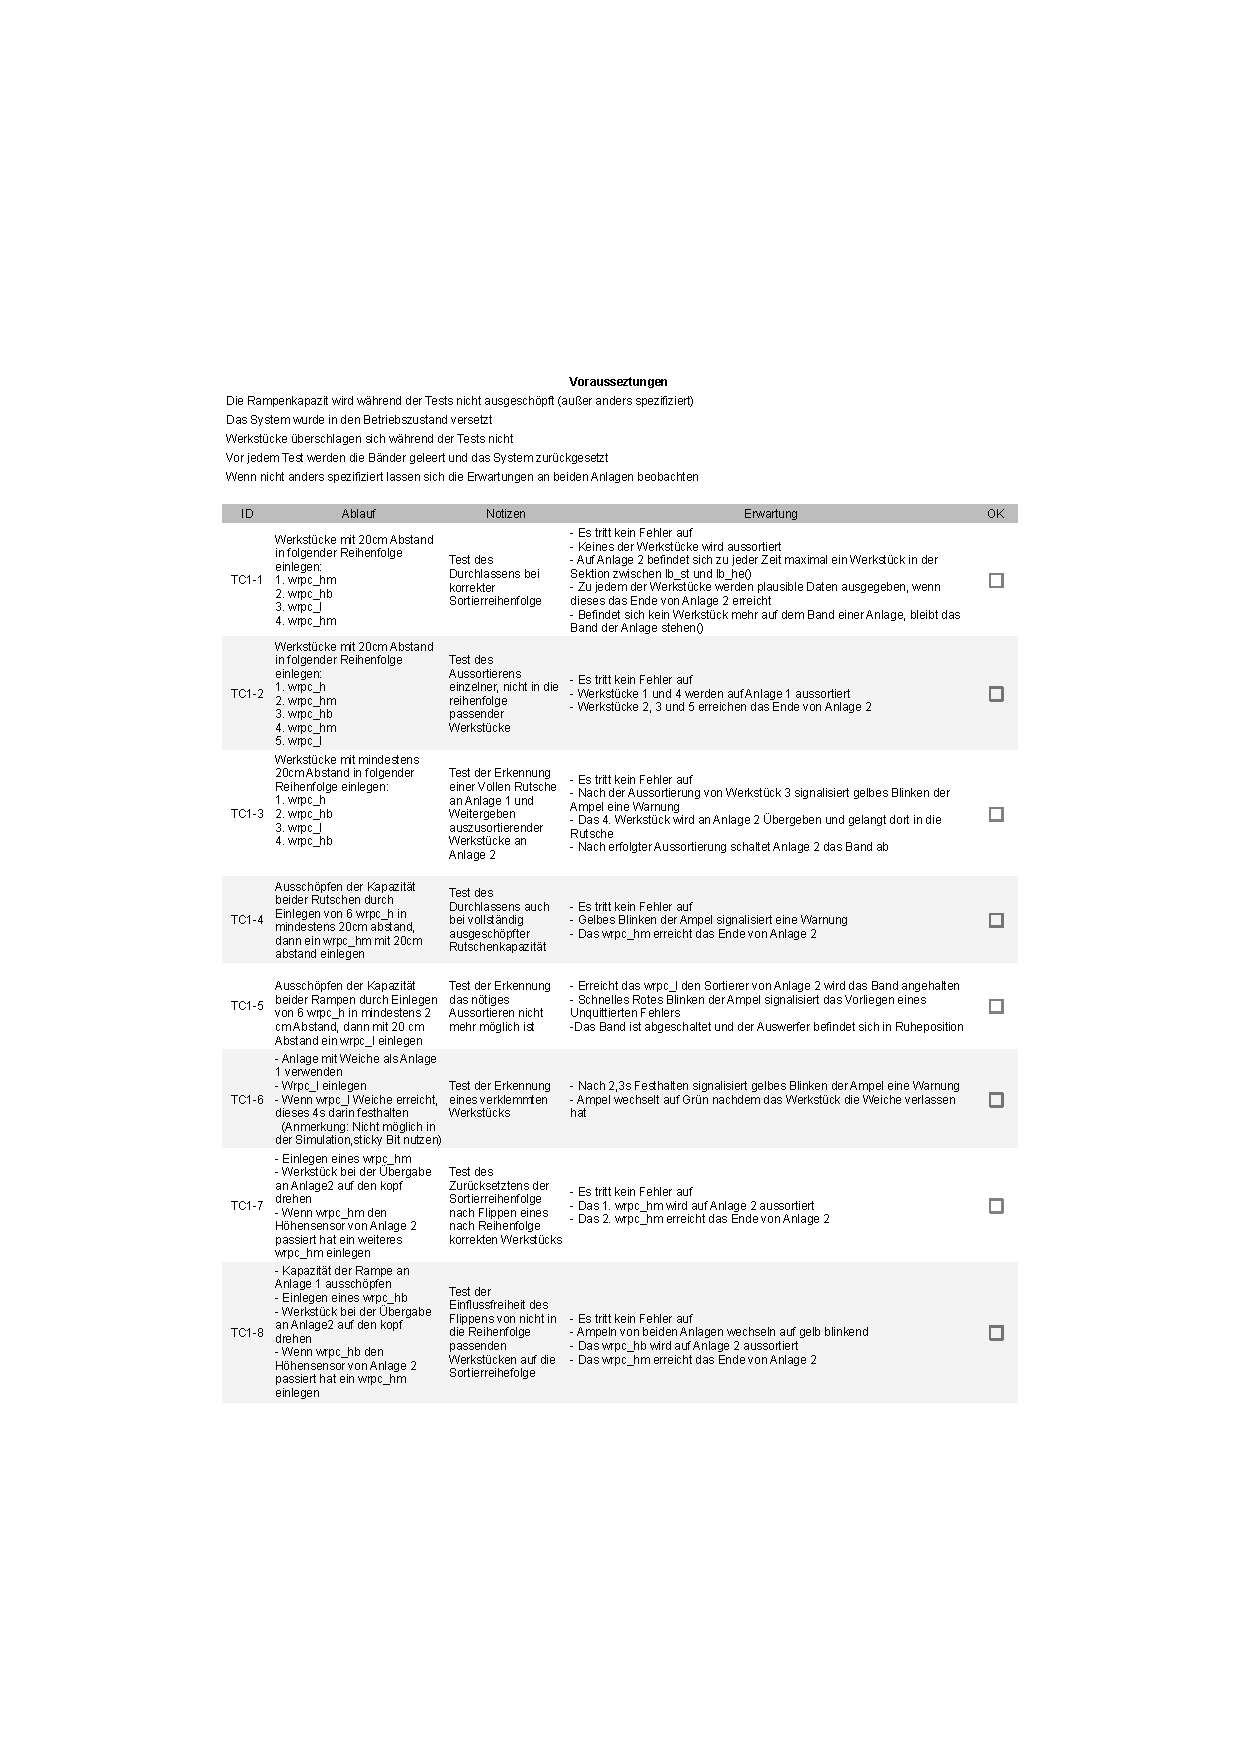
\includepdf[pages={1},pagecommand={ \subsection{Abnahmetest - Sortierung mit Fehlererkennung}}]{anhang/Abnahmetests.pdf}
\includepdf[pages={2},pagecommand={ \subsection{Abnahmetest - Behandlung von Fehlern}}]{anhang/Abnahmetests.pdf}
\includepdf[pages={3},pagecommand={ \subsection{Abnahmetest - Bedienung durch Taster}}]{anhang/Abnahmetests.pdf}
\includepdf[pages={4},pagecommand={ \subsection{Abnahmetest - Eventrecorder}}]{anhang/Abnahmetests.pdf}
\includepdf[pages={5},pagecommand={ \subsection{Abnahmetest - EStop und Verbindungsabbruch}}]{anhang/Abnahmetests.pdf}


\subsection{Ergebnisse der Unit-Tests}\label{subsec:unit-tests-results}
\begin{figure}[H]
    \centering
    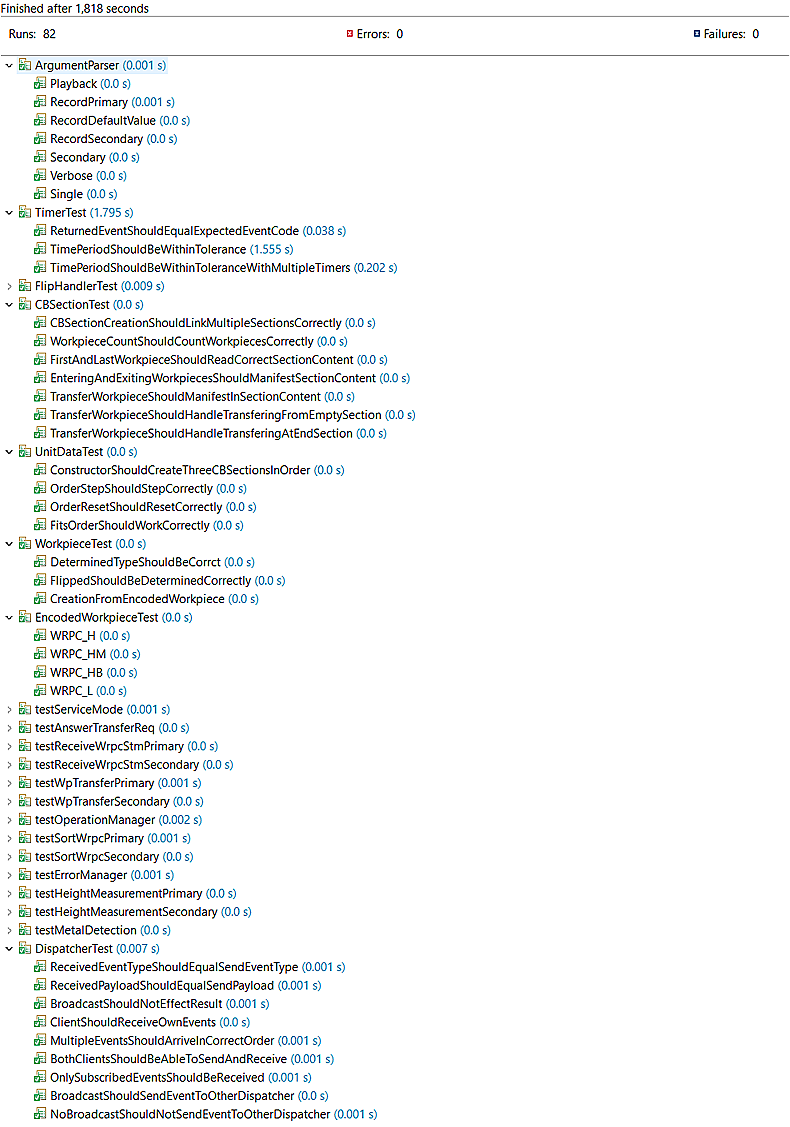
\includegraphics[scale = 0.45]{anhang/unit-test-execution.png}
    \caption{Ergebnisse der Unit-Tests}
    \label{fig:unit-test-execution}
\end{figure}


\subsection{Hal Tests}\label{subsec:hal-tests}

Das Testen der Hal kann kaum automatisiert werden, da beim Test der Aktorik physikalisches Verhalten der Anlage beobachtet werden muss.
Die Sensoriktests erfordern ebenfalls direkte Interaktion mit den Tastern, Lichtschranken, etc.
Daher müssen diese Tests manuell durchgeführt werden.

\subsubsection{Sensorik Tests}\label{subsubsec:sensorik-tests}
Für die durchführung der Tests wird das Logging des Dispatchers verwendet.
Das Ereignis wird ausgeführt und überprüft, ob das richtige Event im Console Logger erscheint.
Zur Erzeugung Lichtschranken- und Metallsensorevents werden verschiedene \gls{workpiece} durch eine \gls{anlage} gefahren.
Bei der Höhenmessung werden \gls{workpiece} unter dem Sensor platziert und der Messwert mit dem für den \gls{workpiece_type}
spezifizierten abgeglichen.

\begin{table}[H]
    \resizebox{\textwidth}{!}{%
    \setlength{\tabcolsep}{20pt}
    \renewcommand{\arraystretch}{1.5}
    \begin{tabular}{|c|c|c|c|}
    \hline
    Ereignis                  & Kommentar                                                                                        & Erw. Event       & Bestanden \\ \hline
    LB\_ST unterbrochen       &                                                                                                  & LB\_ST\_BLCK     & x         \\ \hline
    LB\_ST wieder frei        &                                                                                                  & LB\_ST\_CLR      & x         \\ \hline
    LB\_SW unterbrochen       &                                                                                                  & LB\_SW\_BLCK     & x         \\ \hline
    LB\_SW wieder frei        &                                                                                                  & LB\_SW\_CLR      & x         \\ \hline
    LB\_RA unterbrochen       &                                                                                                  & LB\_RA\_BLCK     & x         \\ \hline
    LB\_RA wieder frei        &                                                                                                  & LB\_RA\_CLR      & x         \\ \hline
    LB\_EN unterbrochen       &                                                                                                  & LB\_EN\_BLCK     & x         \\ \hline
    LB\_EN wieder frei        &                                                                                                  & LB\_EN\_CLR      & x         \\ \hline
    LB\_HE unterbrochen       &                                                                                                  & LB\_HE\_BLCK     & x         \\ \hline
    LB\_HE wieder frei        &                                                                                                  & LB\_HE\_CLR      & x         \\ \hline
    Metall unter Metallsens.  &                                                                                                  & METAL\_DTC       & x         \\ \hline
    Höhenmessung durchgeführt & \begin{tabular}[c]{@{}l@{}}Muss von DemoClient\\ mit HEIGHT\_REQ\\ angefragt werden\end{tabular} & HEIGHT\_HE       & x         \\ \hline
    EStop gedrückt            &                                                                                                  & ESTOP\_ON        & x         \\ \hline
    EStop herausgezogen       &                                                                                                  & ESTOP\_OFF       & x         \\ \hline
    T\_STR kurz drücken       &                                                                                                  & T\_STR\_PRS\_SRT & x         \\ \hline
    T\_STR lang drücken       & \textgreater 3 sec                                                                               & T\_STR\_PRS\_LNG & x         \\ \hline
    T\_STP kurz drücken       &                                                                                                  & T\_STP\_PRS\_SRT & x         \\ \hline
    T\_STP lang drücken       & \textgreater 3 sec                                                                               & T\_STP\_PRS\_LNG & x         \\ \hline
    T\_RST kurz drücken       &                                                                                                  & T\_RST\_PRS\_LNG & x         \\ \hline
    T\_RST lang drücken       & \textgreater 3 sec                                                                               & T\_RST\_PRS\_SRT & x         \\ \hline
    \end{tabular}}
    \end{table}


\subsubsection{Aktorik Tests}\label{subsubsec:aktorik-tests}
Für die Durchführung der Tests wird ein spezieller DispatcherClient (DemoClient)
benutzt, der beim Drücken auf die Knöpfe am Bedienfeld der Anlage wählbare zur Compilezeit
wählbare Events an den Dispatcher schickt. Die Reaktion der Aktorik auf diese Events wird beobachtet.
Die Events sind hier ohne das Prefix EVNT\_ACT aufgelistet.

\begin{table}[H]
    \resizebox{\textwidth}{!}{%
    \setlength{\tabcolsep}{20pt}
    \renewcommand{\arraystretch}{1.5}
    \begin{tabular}{|c|c|c|c|}
    \hline
    Event                             & Kommentar          & Erwartetes Ereignis         & Bestanden \\ \hline
    CTRL\_T\_STR\_LED\_ON  &                    & LED T\_STR an               & x         \\ \hline
    CTRL\_T\_STR\_LED\_OFF &                    & LED T\_SRT aus              & x         \\ \hline
    CTRL\_T\_RST\_LED\_ON  &                    & LED T\_RST an               & x         \\ \hline
    CTRL\_T\_RST\_LED\_OFF &                    & LED T\_RST aus              & x         \\ \hline
    SORT\_DSC              & Mit Weiche         & Weiche in Auswerfpos.       & x         \\ \hline
    SORT\_NO\_DSC          & Mit Weiche         & Weiche in Durchlasspos.     & x         \\ \hline
    SORT\_RST              & Mit Weiche         & Weiche in Auswerfpos.       & x         \\ \hline
    SORT\_DSC              & Mit Pusher         & Pusher ausgefahren          & x         \\ \hline
    SORT\_NO\_DSC          & Mit Pusher         & Pusher eingefahren          & x         \\ \hline
    SORT\_RST              & Mit Pusher         & Pusher eingefahren          & x         \\ \hline
    BELT\_FWD              &                    & Band fährt vorwärts         & x         \\ \hline
    BELT\_BWD              &                    & Band fährt rückwärts        & x         \\ \hline
    BELT\_STP              &                    & Band hält an                & x         \\ \hline
    STPL\_LED\_ON          & Alle Farben testen & Ampelfarbe geht an          & x         \\ \hline
    STPL\_LED\_OFF         & Alle Farben testen & Ampelfarbe geht wieder aus  & x         \\ \hline
    STPL\_LED\_BLNK\_FST   & Alle Farben testen & Ampelfarbe blinkt mit 1Hz   & x         \\ \hline
    STPL\_LED\_BLNK\_SLW   & Alle Farben testen & Ampelfarbe blinkt mit 0.5Hz & x         \\ \hline
    \end{tabular}}
    \end{table}
